\documentclass[main]{subfiles}
\begin{document}

%@@@@@@@@@@@@@@@@@@@@@@@@@@@@@@
% Main Topics: Perceptron Learning Algorithm 06.12.2018
% Lecturer: Matthew Cook
% author: Vanessa Leite - base document from benelot/eth-intro-to-neuroinformatics-summary

\section{Interacting Neural Populations}

\subsubsection{Perceptive Visual Field}

A neuron is "tuned" to a moving bar at a certani angle in its perceptive field. It also responds to a certain velocity, position (x,y), bar width, etc.

Neurons response is called firing rates. Although neurons are tuned, they aren't super picky about the exact values. And, experimentally, neurons do not code a single atributte but a combination of them.

\paragraph{Population code}

Information is encoded by a group (population) of neurons. A group includes all neurons in that area. The values are encoded by pattern of activity.

\begin{itemize}[noitemsep,nolistsep]
	\item Neurons can represent information through population codes.
	\item Neurons are tuned to preferred stimuli.
	\item Information is represented by the pattern of activity in a neural population.
	\item Each neuron has a preferred input, for example orientation, that it responds to. The neuron is tuned to that value.
	\item Not every neuron shows clear tuning curves.
	\item Neurons usually do not only respond to their preferred stimulus, but also with decaying strength to close ones.
\end{itemize}

\begin{figure}[H]
	\centering
	\begin{subfigure}[b]{0.3\textwidth}
		\centering
		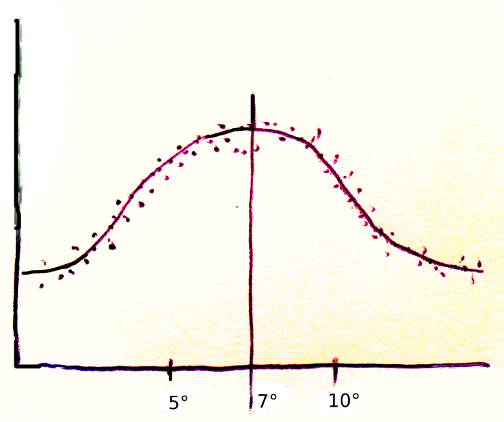
\includegraphics[width=\textwidth]{one-cell-tuning-curve.png}
		\caption{Tuning curve of one cell}
	\end{subfigure}%
	~
	\begin{subfigure}[b]{0.3\textwidth}
		\centering
		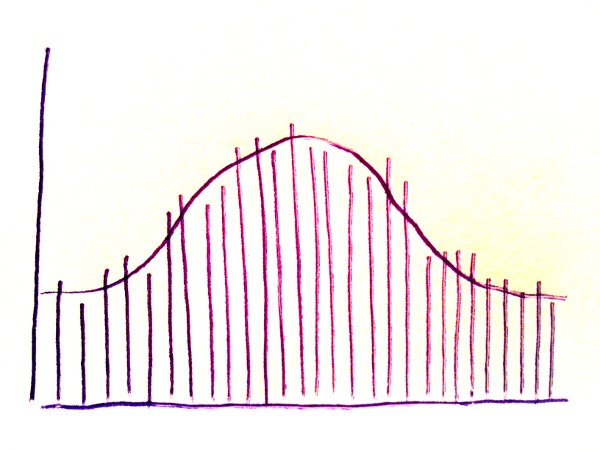
\includegraphics[width=\textwidth]{cell-order.png}
		\caption{Cells ordered by response to $20^\circ$}
	\end{subfigure}
	~ 
	\begin{subfigure}[b]{0.3\textwidth}
		\centering
		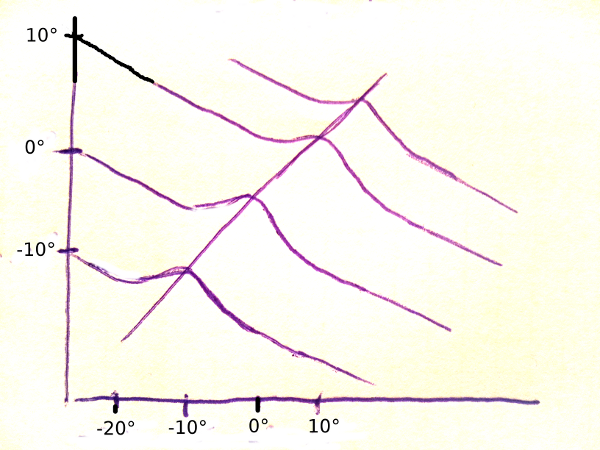
\includegraphics[width=\textwidth]{3D-visualisation.png}
		\caption{3D visualization of cell's response to different degrees}
	\end{subfigure}
\end{figure}

\begin{figure}[H]
	\centering
	\begin{subfigure}[b]{0.5\textwidth}
		\centering
		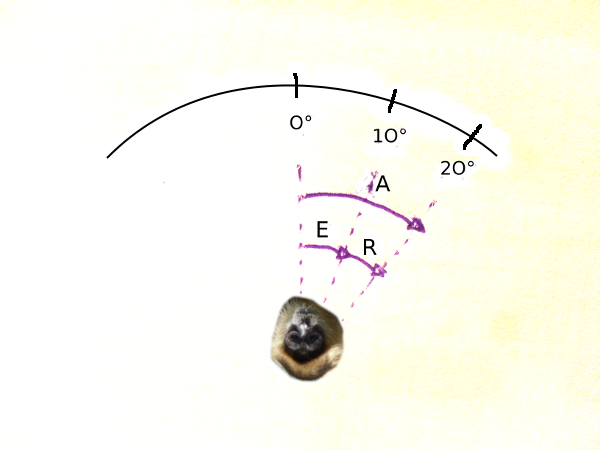
\includegraphics[width=\textwidth]{ape-picture.png}
		\caption{Monkey holding gaze fixed on point $10^\circ$ and light falling in from $20^\circ$}
	\end{subfigure}%
	~
	\begin{subfigure}[b]{0.5\textwidth}
		\centering
		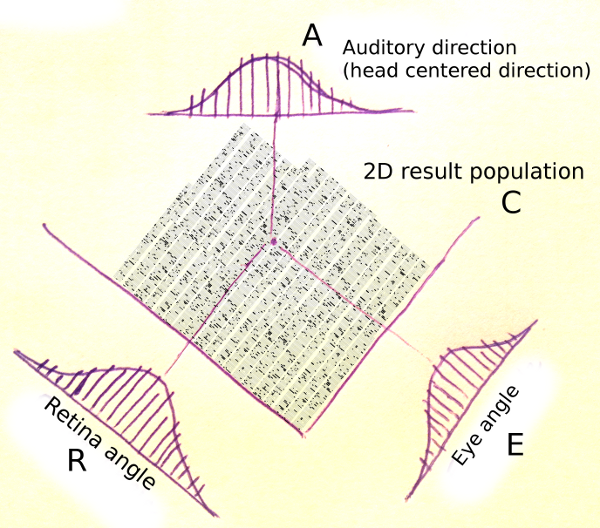
\includegraphics[width=\textwidth]{Retina-Eye-Auditory.png}
		\caption{Visualization of Retina angle ordering cell set R, Eye angle ordering set E,2D result population C and auditory direction set A.}
		\label{fig:population}
	\end{subfigure}
\end{figure}

\begin{figure}[H]
	\centering
	\begin{subfigure}[b]{0.3\textwidth}
		\centering
		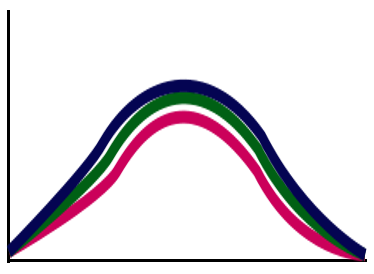
\includegraphics[width=\textwidth]{Cell-A.png}
		\caption{Cell A $\in$ R}
	\end{subfigure}%
	~
	\begin{subfigure}[b]{0.3\textwidth}
		\centering
		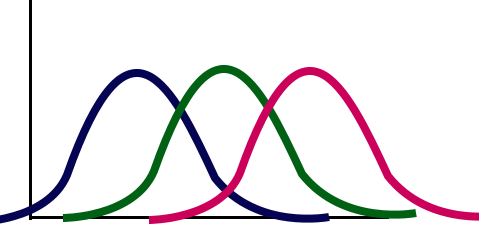
\includegraphics[width=\textwidth]{Cell-B.png}
		\caption{Cell B $\in$ A}
	\end{subfigure}
	~ 
	\begin{subfigure}[b]{0.3\textwidth}
		\centering
		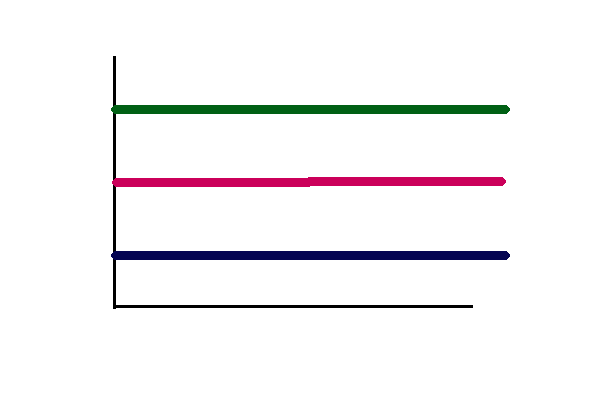
\includegraphics[width=\textwidth]{Cell-C.png}
		\caption{Cell C $\in$ E}
	\end{subfigure}
\end{figure}

\begin{figure}[H]
	\centering
	\begin{subfigure}[b]{0.3\textwidth}
		\centering
		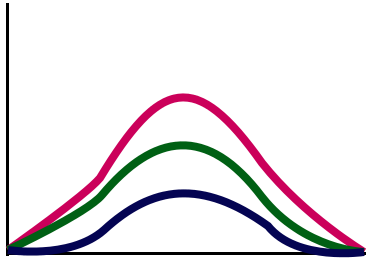
\includegraphics[width=\textwidth]{Cell-D.png}
		\caption{Cell D $\in$ C}
	\end{subfigure}%
	~
	\begin{subfigure}[b]{0.3\textwidth}
		\centering
		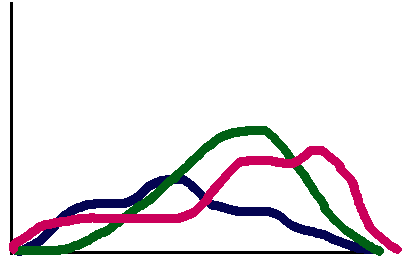
\includegraphics[width=\textwidth]{Cell-E.png}
		\caption{Cell E (Not every neuron shows clear tuning curves)}
	\end{subfigure}
\end{figure}

$R$, $A$ and $E$ have the following relations:
\begin{itemize}
\item $R = A - E$
\item $A = E + R$
\item $E = A - R$
\end{itemize}

How does this information is stored? Say $R$, $A$ and $E$ are encoded by population codes, i.e., by population of units, each tuned to a particular value of that variable. Considering these three variables, the result is seen in Figure~\ref{fig:population}.


\end{document}
